\documentclass[aspectratio=169,11pt]{beamer}

\usetheme{Madrid}
\usecolortheme{default}
\setbeamertemplate{navigation symbols}{}
\setbeamertemplate{footline}[frame number]

\usepackage[utf8]{inputenc}
\usepackage[T1]{fontenc}
\usepackage{lmodern}
\usepackage{amsmath,amssymb}
\usepackage{booktabs}
\usepackage{array}
\usepackage{tabularx}
\usepackage{makecell}
\usepackage{tikz}
\usetikzlibrary{arrows.meta,positioning,fit,shapes.geometric}

\definecolor{ozublue}{RGB}{20,63,122}
\definecolor{ozugray}{RGB}{80,85,95}
\definecolor{lightblue}{RGB}{231,240,253}
\definecolor{lightgray}{RGB}{245,246,248}
\setbeamercolor{structure}{fg=ozublue}
\setbeamercolor{frametitle}{fg=white,bg=ozublue}
\setbeamercolor{title}{fg=white,bg=ozublue}
\setbeamercolor{block title}{fg=white,bg=ozublue}
\setbeamercolor{block body}{bg=lightgray}

\newcolumntype{Y}{>{\raggedright\arraybackslash}X}
\newcommand{\tcssop}{\textsc{TCSSOP}}
\newcommand{\eval}{\mathrm{Eval}}

\title[Tez İzleme Sunumu]{Entegre Numune Sayısı Optimizasyonu ve Çevresel Kısıtlar Altında Test Odası Çizelgeleme}
\subtitle{Tez İzleme Sunumu}
\author[N. Perçin]{Nur Perçin\\\small Danışman: Prof. Dr. Ali Ekici}
\institute[ÖzÜ]{Özyeğin Üniversitesi\\Endüstri Mühendisliği Bölümü}
\date{\today}

\begin{document}

\begin{frame}
  \titlepage
\end{frame}

\begin{frame}{Sunum Akışı}
  \tableofcontents
\end{frame}

\section{Motivasyon ve Problem Bağlamı}

\begin{frame}{Endüstriyel Motivasyon}
  \begin{block}{R\&D test sürecinin kritik rolü}
    Buzdolabı ürünleri pazara çıkmadan önce enerji, performans, güvenlik ve kullanım testlerinden geçmek zorundadır.
  \end{block}

  \begin{columns}[T,totalwidth=\textwidth]
    \begin{column}{0.48\textwidth}
      \textbf{Operasyonel baskılar}
      \begin{itemize}
        \item Kısa ürün geliştirme çevrimleri
        \item Sıkı lansman ve sertifikasyon tarihleri
        \item Sermaye yoğun test altyapısı
        \item Heterojen test odaları ve istasyonlar
      \end{itemize}
    \end{column}
    \begin{column}{0.48\textwidth}
      \textbf{Planlama zorlukları}
      \begin{itemize}
        \item Sıcaklık, nem ve voltaj uygunluğu
        \item Ürün bazlı test gereksinimleri
        \item Aşama bağımlı süreç mantığı
        \item Numune sayısına bağlı iş yükü
      \end{itemize}
    \end{column}
  \end{columns}

  \vspace{2mm}
  \alert{Temel soru:} Sabit numune politikası yerine numune sayısı karar değişkeni yapılırsa toplam gecikme azaltılabilir mi?
\end{frame}

\begin{frame}{Test Odası Sistemi}
  \begin{columns}[T,totalwidth=\textwidth]
    \begin{column}{0.55\textwidth}
      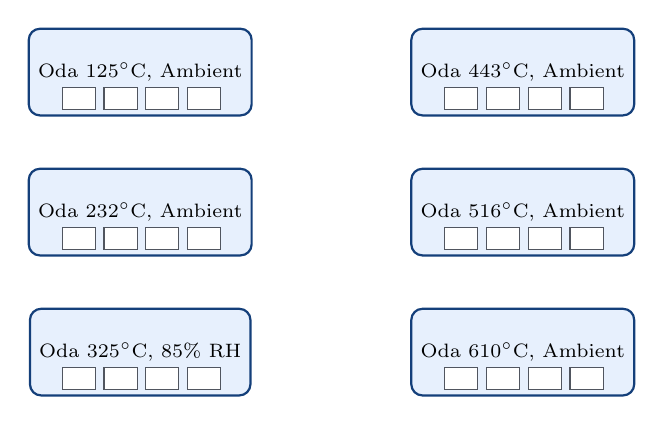
\begin{tikzpicture}[
        chamber/.style={draw=ozublue,thick,rounded corners,fill=lightblue,minimum width=2.7cm,minimum height=1.1cm},
        station/.style={draw=ozugray,fill=white,minimum width=0.42cm,minimum height=0.28cm},
        every node/.style={font=\scriptsize}
      ]
        \node[chamber] (c1) {Oda 1\\$25^\circ$C, Ambient};
        \node[chamber,below=0.65cm of c1] (c2) {Oda 2\\$32^\circ$C, Ambient};
        \node[chamber,below=0.65cm of c2] (c3) {Oda 3\\$25^\circ$C, 85\% RH};
        \node[chamber,right=2.0cm of c1] (c4) {Oda 4\\$43^\circ$C, Ambient};
        \node[chamber,below=0.65cm of c4] (c5) {Oda 5\\$16^\circ$C, Ambient};
        \node[chamber,below=0.65cm of c5] (c6) {Oda 6\\$10^\circ$C, Ambient};

        \foreach \c in {c1,c2,c3,c4,c5,c6}{
          \node[station] at ([xshift=-0.78cm,yshift=-0.34cm]\c.center) {};
          \node[station] at ([xshift=-0.25cm,yshift=-0.34cm]\c.center) {};
          \node[station] at ([xshift=0.28cm,yshift=-0.34cm]\c.center) {};
          \node[station] at ([xshift=0.81cm,yshift=-0.34cm]\c.center) {};
        }
      \end{tikzpicture}
    \end{column}
    \begin{column}{0.42\textwidth}
      \textbf{Yapısal özellikler}
      \begin{itemize}
        \item Her odada birden çok paralel istasyon vardır.
        \item Aynı odadaki istasyonlar ortak çevresel ayarda çalışır.
        \item Nem ve voltaj kabiliyetleri odalar arasında farklıdır.
        \item Testler sadece uyumlu çevre ve kabiliyete sahip odalara atanabilir.
      \end{itemize}
    \end{column}
  \end{columns}
\end{frame}

\begin{frame}{Test Akışı ve Numune Etkisi}
  \begin{center}
    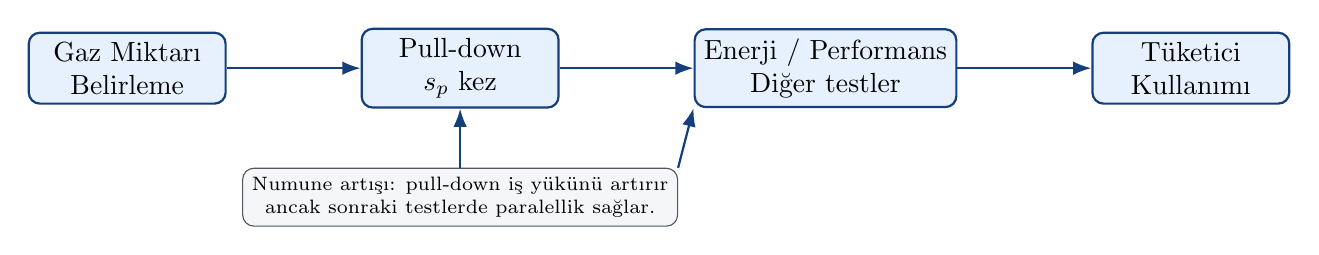
\begin{tikzpicture}[
      node distance=1.7cm,
      box/.style={draw=ozublue,thick,rounded corners,fill=lightblue,align=center,minimum width=2.5cm,minimum height=0.9cm},
      arrow/.style={-Latex,thick,draw=ozublue},
      note/.style={draw=ozugray,rounded corners,fill=lightgray,align=center,font=\scriptsize}
    ]
      \node[box] (gas) {Gaz Miktarı\\Belirleme};
      \node[box,right=of gas] (pull) {Pull-down\\$s_p$ kez};
      \node[box,right=of pull] (other) {Enerji / Performans\\Diğer testler};
      \node[box,right=of other] (usage) {Tüketici\\Kullanımı};

      \draw[arrow] (gas) -- (pull);
      \draw[arrow] (pull) -- (other);
      \draw[arrow] (other) -- (usage);

      \node[note,below=0.75cm of pull] (trade) {
        Numune artışı: pull-down iş yükünü artırır\\
        ancak sonraki testlerde paralellik sağlar.
      };
      \draw[arrow] (trade.north) -- (pull.south);
      \draw[arrow] (trade.north east) -- (other.south west);
    \end{tikzpicture}
  \end{center}

  \[
  m_{pt}(s_p)=
  \begin{cases}
  s_p, & \text{pull-down testi ise},\\
  1, & \text{diğer testler için}.
  \end{cases}
  \]

  \begin{block}{Karar-bağımlı iş yükü}
    Numune sayısı yalnızca kaynak tüketimini değil, çizelgenin paralelleşme kapasitesini de değiştirir.
  \end{block}
\end{frame}

\section{Araştırma Boşluğu ve Katkı}

\begin{frame}{Literatürde Konumlandırma}
  \begin{tabularx}{\textwidth}{p{0.27\textwidth}Y Y}
    \toprule
    \textbf{Literatür alanı} & \textbf{Tipik odak} & \textbf{Bu çalışmadaki boşluk} \\
    \midrule
    Kaynak kısıtlı çok projeli çizelgeleme & Sabit faaliyet kümesi, öncelikler, kaynaklar & İş yükü karar değişkenlerinden türemiyor. \\
    \addlinespace
    Paralel makine çizelgeleme & Makine uygunluğu, gecikme, atama ve sıralama & Çevresel oda konfigürasyonu ve numune mantığı birlikte ele alınmıyor. \\
    \addlinespace
    Sipariş kabul ve çizelgeleme & Hangi işlerin seçileceği ve ne zaman yapılacağı & İşlerin sayısı/yoğunluğu numune kararıyla oluşmuyor. \\
    \addlinespace
    Güvenilirlik/test planlama & Numune sayısı, test süresi, risk & Detaylı kaynak kısıtlı yürütme çizelgesi genellikle yok. \\
    \bottomrule
  \end{tabularx}

  \vspace{3mm}
  \alert{Araştırma boşluğu:} Numune sayısı, oda konfigürasyonu ve kaynak kısıtlı çizelgeleme kararlarının birlikte modellenmesi.
\end{frame}

\begin{frame}{Çalışmanın Katkıları}
  \begin{enumerate}
    \item \textbf{Yeni problem yapısı:} Test Chamber Scheduling with Sample Optimization Problem (\tcssop).
    \item \textbf{Karar-bağımlı iş yükü:} Numune sayısı sabit parametre değil, optimizasyon değişkenidir.
    \item \textbf{Entegre çözüm yaklaşımı:} Oda çevre ataması, numune optimizasyonu ve çizelgeleme geri beslemeli yürütülür.
    \item \textbf{VNS tabanlı çeşitlendirme:} Sıralama yerine iş yükünü tanımlayan numune vektörü pertürbe edilir.
    \item \textbf{Feasibility assurance:} Çevre, nem, voltaj, istasyon, numune ve aşama mantığı ayrı doğrulanır.
  \end{enumerate}
\end{frame}

\section{Problem Tanımı}

\begin{frame}{TCSSOP: Karar Bileşenleri}
  \begin{columns}[T,totalwidth=\textwidth]
    \begin{column}{0.33\textwidth}
      \begin{block}{1. Oda konfigürasyonu}
        \[
        X_c \in \mathcal{E}
        \]
        Her oda için sıcaklık--nem ortamı belirlenir.
      \end{block}
    \end{column}
    \begin{column}{0.33\textwidth}
      \begin{block}{2. Numune sayısı}
        \[
        s_{\min}\le s_p\le s_{\max}
        \]
        Her ürün için fiziksel numune sayısı seçilir.
      \end{block}
    \end{column}
    \begin{column}{0.33\textwidth}
      \begin{block}{3. Çizelgeleme}
        \[
        \Pi = \{(p,t,k,start,finish)\}
        \]
        Testler uyumlu oda istasyonlarına zamanlanır.
      \end{block}
    \end{column}
  \end{columns}

  \vspace{3mm}
  \begin{center}
    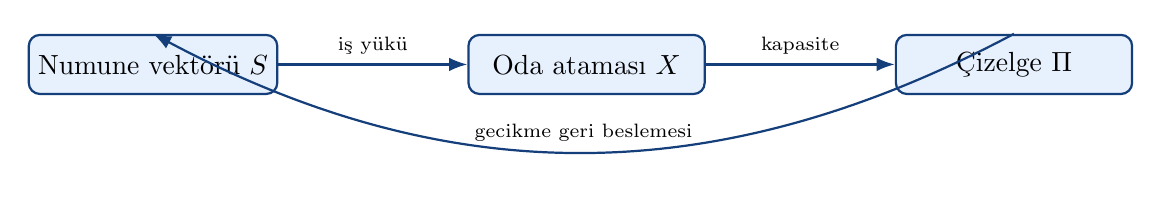
\begin{tikzpicture}[
      node distance=2.4cm,
      box/.style={draw=ozublue,rounded corners,thick,fill=lightblue,align=center,minimum width=3cm,minimum height=0.75cm},
      arrow/.style={-Latex,thick,draw=ozublue}
    ]
      \node[box] (samples) {Numune vektörü $S$};
      \node[box,right=of samples] (assign) {Oda ataması $X$};
      \node[box,right=of assign] (schedule) {Çizelge $\Pi$};
      \draw[arrow] (samples) -- node[above,font=\scriptsize]{iş yükü} (assign);
      \draw[arrow] (assign) -- node[above,font=\scriptsize]{kapasite} (schedule);
      \draw[arrow,bend left=28] (schedule.north) to node[above,font=\scriptsize]{gecikme geri beslemesi} (samples.north);
    \end{tikzpicture}
  \end{center}
\end{frame}

\begin{frame}{Amaç Fonksiyonu ve Önceliklendirme}
  \begin{block}{Birincil amaç: toplam gecikme}
    \[
    T_p=\max(0,C_p-d_p), \qquad
    T^{tot}=\sum_{p\in\mathcal{P}}T_p
    \]
  \end{block}

  \begin{block}{İkincil amaç: toplam numune kullanımı}
    \[
    S^{tot}=\sum_{p\in\mathcal{P}}s_p
    \]
  \end{block}

  \begin{alertblock}{Leksikografik değerlendirme}
    \[
    \eval=(T^{tot},S^{tot})
    \]
    Önce toplam gecikme minimize edilir; eşit gecikmede daha az numune kullanan çözüm tercih edilir.
  \end{alertblock}
\end{frame}

\begin{frame}{Temel Fizibilite Koşulları}
  \begin{columns}[T,totalwidth=\textwidth]
    \begin{column}{0.49\textwidth}
      \textbf{Yapısal uygunluk}
      \begin{itemize}
        \item Ürün bazlı gerekli testlerin tamamlanması
        \item Pull-down için $s_p$ operasyon, diğer testler için tek operasyon
        \item Test--oda çevre eşleşmesi
        \item Nem kontrollü testler için nem kabiliyeti
        \item Voltaj gerektiren ürünler için voltaj uyumlu odalar
      \end{itemize}
    \end{column}
    \begin{column}{0.49\textwidth}
      \textbf{Zamansal uygunluk}
      \begin{itemize}
        \item Her istasyonda aynı anda en fazla bir test
        \item Aynı numunede test çakışmaması
        \item Aşama-durumu öncelik mantığı
        \item Ürün tamamlanma zamanının son test bitişiyle belirlenmesi
        \item Numune alt ve üst sınırları
      \end{itemize}
    \end{column}
  \end{columns}
\end{frame}

\section{Çözüm Metodolojisi}

\begin{frame}{Genel Çözüm Çerçevesi}
  \begin{center}
    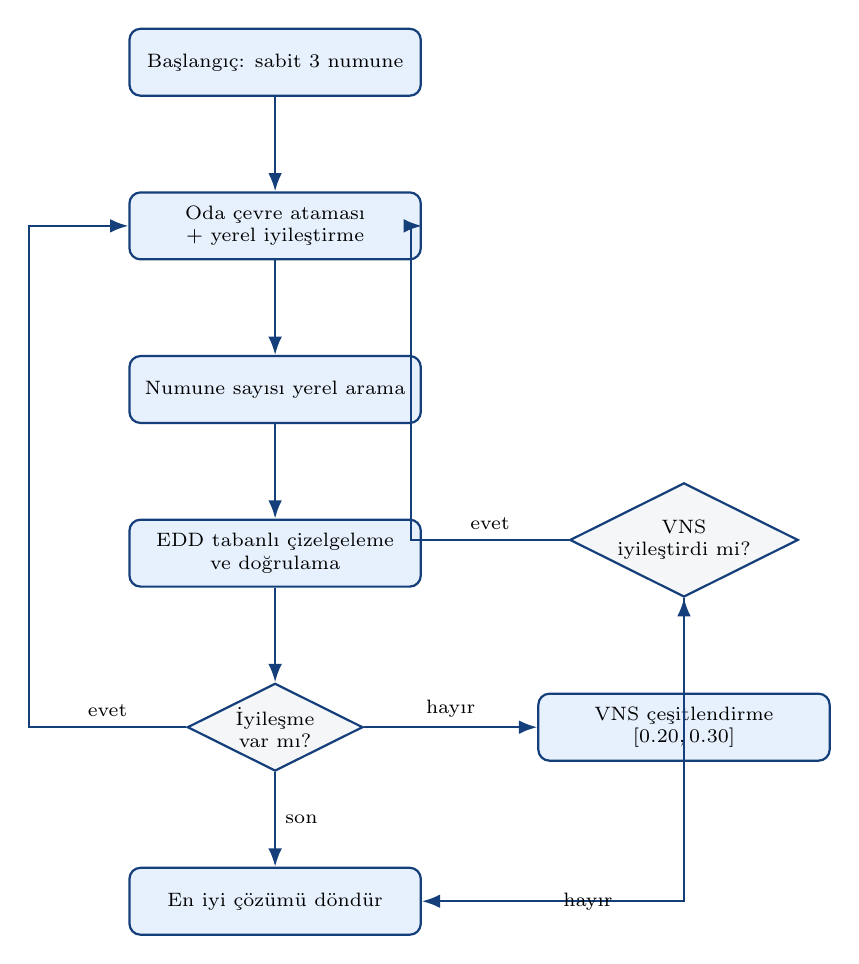
\begin{tikzpicture}[
      node distance=1.2cm and 1.5cm,
      box/.style={draw=ozublue,thick,rounded corners,fill=lightblue,align=center,minimum width=3.7cm,minimum height=0.85cm},
      decision/.style={draw=ozublue,thick,diamond,aspect=2.0,fill=lightgray,align=center,inner sep=1pt},
      arrow/.style={-Latex,thick,draw=ozublue},
      every node/.style={font=\scriptsize}
    ]
      \node[box] (init) {Başlangıç: sabit 3 numune};
      \node[box,below=of init] (assign) {Oda çevre ataması\\+ yerel iyileştirme};
      \node[box,below=of assign] (sample) {Numune sayısı yerel arama};
      \node[box,below=of sample] (sched) {EDD tabanlı çizelgeleme\\ve doğrulama};
      \node[decision,below=of sched] (imp) {İyileşme\\var mı?};
      \node[box,right=2.2cm of imp] (vns) {VNS çeşitlendirme\\$[0.20,0.30]$};
      \node[decision,above=of vns] (vimp) {VNS\\iyileştirdi mi?};
      \node[box,below=of imp] (stop) {En iyi çözümü döndür};

      \draw[arrow] (init) -- (assign);
      \draw[arrow] (assign) -- (sample);
      \draw[arrow] (sample) -- (sched);
      \draw[arrow] (sched) -- (imp);
      \draw[arrow] (imp.east) -- node[above]{hayır} (vns.west);
      \draw[arrow] (vns) -- (vimp);
      \draw[arrow] (vimp.west) -- node[above]{evet} ++(-2.0,0) |- (assign.east);
      \draw[arrow] (imp.west) -- node[above]{evet} ++(-2.0,0) |- (assign.west);
      \draw[arrow] (vimp.south) |- node[pos=0.75,right]{hayır} (stop.east);
      \draw[arrow] (imp) -- node[right]{son} (stop);
    \end{tikzpicture}
  \end{center}
\end{frame}

\begin{frame}{Aşama 1: Oda Çevre Ataması}
  \begin{block}{İş yükü tahmini}
    \[
    W_e(S)=\sum_{p\in\mathcal{P}}
    \sum_{\substack{t\in\mathcal{T}_p\\e(t)=e}}
    m_{pt}(S)\tau_t
    \]
  \end{block}

  \begin{columns}[T,totalwidth=\textwidth]
    \begin{column}{0.48\textwidth}
      \textbf{Exact model}
      \begin{itemize}
        \item Her oda tek çevreye atanır.
        \item Her çevre en az bir oda alır.
        \item Nem uygunluğu zorunludur.
        \item Kapasite, iş yükü paylarına göre dengelenir.
      \end{itemize}
    \end{column}
    \begin{column}{0.48\textwidth}
      \textbf{Yerel iyileştirme}
      \begin{itemize}
        \item \textit{Swap}: iki odanın çevrelerini değiştirir.
        \item \textit{Move}: bir odayı başka çevreye taşır.
        \item Hızlı çizelge-duyarlı değerlendirme kullanılır.
      \end{itemize}
    \end{column}
  \end{columns}
\end{frame}

\begin{frame}{Aşama 2: Numune Sayısı Optimizasyonu}
  \begin{columns}[T,totalwidth=\textwidth]
    \begin{column}{0.52\textwidth}
      \textbf{Yerel arama hareketleri}
      \[
      \Delta_p\subseteq\{-2,-1,+1,+2\}
      \]
      \begin{itemize}
        \item Her ürün için sınır içi numune değişimleri denenir.
        \item Adaylar önce hızlı değerlendirme ile elenir.
        \item Kabul edilen hareketler tam çizelgeleme ile doğrulanır.
      \end{itemize}
    \end{column}
    \begin{column}{0.45\textwidth}
      \textbf{Late--Early rebalance}
      \begin{itemize}
        \item Geciken ürünlerde numune artırma eğilimi
        \item Erken biten ürünlerde numune azaltma eğilimi
        \item Toplam gecikmeyi kötüleştirmeyen hareket kabul edilir.
      \end{itemize}
    \end{column}
  \end{columns}

  \vspace{3mm}
  \begin{alertblock}{Temel sezgi}
    Numuneyi azaltmak iş yükünü düşürür; numuneyi artırmak ise bazı ürünlerde paralelliği artırarak tamamlanma zamanını düşürebilir.
  \end{alertblock}
\end{frame}

\begin{frame}{Çizelgeleme Prosedürü}
  \begin{columns}[T,totalwidth=\textwidth]
    \begin{column}{0.50\textwidth}
      \textbf{EDD tabanlı hazır-küme çizelgeleme}
      \begin{enumerate}
        \item Her ürün için aşama durumuna göre hazır operasyon aranır.
        \item Uygun oda, istasyon ve numune kombinasyonu bulunur.
        \item Küresel aday havuzundan en erken teslim tarihli iş seçilir.
        \item Sistem durumu güncellenir.
      \end{enumerate}
    \end{column}
    \begin{column}{0.47\textwidth}
      \textbf{Dinamik hazır olma koşulları}
      \begin{itemize}
        \item Gas tamamlanmadan pull-down başlamaz.
        \item Diğer testler pull-down fazından sonra açılır.
        \item Tüketici kullanımı, diğer testlerin başlaması ve pull-down bitişine bağlıdır.
        \item Aynı numune iki eşzamanlı teste giremez.
      \end{itemize}
    \end{column}
  \end{columns}
\end{frame}

\begin{frame}{VNS Tabanlı Çeşitlendirme}
  \begin{center}
    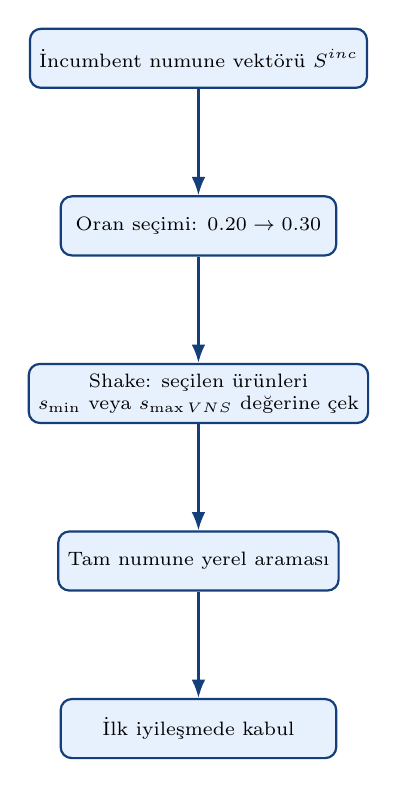
\begin{tikzpicture}[
      node distance=1.35cm,
      box/.style={draw=ozublue,thick,rounded corners,fill=lightblue,align=center,minimum width=3.5cm,minimum height=0.75cm},
      arrow/.style={-Latex,thick,draw=ozublue},
      every node/.style={font=\scriptsize}
    ]
      \node[box] (inc) {İncumbent numune vektörü $S^{inc}$};
      \node[box,below=of inc] (ratio) {Oran seçimi: $0.20 \rightarrow 0.30$};
      \node[box,below=of ratio] (shake) {Shake: seçilen ürünleri\\$s_{\min}$ veya $s_{\max VNS}$ değerine çek};
      \node[box,below=of shake] (ls) {Tam numune yerel araması};
      \node[box,below=of ls] (accept) {İlk iyileşmede kabul};
      \draw[arrow] (inc) -- (ratio);
      \draw[arrow] (ratio) -- (shake);
      \draw[arrow] (shake) -- (ls);
      \draw[arrow] (ls) -- (accept);
    \end{tikzpicture}
  \end{center}

  \begin{block}{Ayırt edici özellik}
    VNS, klasik olarak sıralama/atama kararlarını değil, problemdeki iş yükünü oluşturan numune kararlarını pertürbe eder.
  \end{block}
\end{frame}

\section{Deneysel Tasarım ve Sonuçlar}

\begin{frame}{Deneysel Tasarım}
  \begin{columns}[T,totalwidth=\textwidth]
    \begin{column}{0.33\textwidth}
      \begin{block}{Test matrisi}
        \begin{itemize}
          \item 10 farklı portföy
          \item Enerji, performans ve opsiyonel test kombinasyonları
          \item Çevre bazlı iş yükü dağılımı
        \end{itemize}
      \end{block}
    \end{column}
    \begin{column}{0.33\textwidth}
      \begin{block}{Teslim tarihi}
        \begin{itemize}
          \item 3 senaryo
          \item Sıkı, orta, gevşek planlama rejimleri
          \item Farklı yayılım seviyeleri
        \end{itemize}
      \end{block}
    \end{column}
    \begin{column}{0.33\textwidth}
      \begin{block}{Voltaj yoğunluğu}
        \begin{itemize}
          \item 3 senaryo
          \item Düşük, orta, yüksek voltaj gereksinimi
          \item Kaynak uygunluğu daralması
        \end{itemize}
      \end{block}
    \end{column}
  \end{columns}

  \vspace{3mm}
  \begin{center}
    \Large
    $10 \times 3 \times 3 = 90$ benchmark senaryosu
  \end{center}
\end{frame}

\begin{frame}{Karşılaştırılan Yöntemler}
  \begin{tabularx}{\textwidth}{p{0.25\textwidth}Y}
    \toprule
    \textbf{Yöntem} & \textbf{Açıklama} \\
    \midrule
    Fixed Sample & Her ürün için sabit $s_p=3$; numune optimizasyonu yok. \\
    \addlinespace
    SO-noOuter & Numune optimizasyonu var; oda konfigürasyonu başlangıçtan sonra güncellenmiyor. \\
    \addlinespace
    SO-noVNS & Numune optimizasyonu ve dış döngü var; VNS çeşitlendirme yok. \\
    \addlinespace
    Önerilen yöntem & Numune optimizasyonu, iteratif oda yeniden ataması ve VNS çeşitlendirme birlikte kullanılır. \\
    \bottomrule
  \end{tabularx}
\end{frame}

\begin{frame}{Parametre Ayarları}
  \begin{table}
    \centering
    \small
    \begin{tabular}{lll}
      \toprule
      \textbf{Parametre} & \textbf{Açıklama} & \textbf{Değer} \\
      \midrule
      $s_p^{(0)}$ & Başlangıç numune politikası & 3 \\
      $s_{\min}$ & Minimum numune sayısı & 3 \\
      $s_{\max VNS}$ & VNS UP hareketi üst değeri & 8 \\
      $s_{\max}$ & Maksimum numune sayısı & 11 \\
      $\Delta_p$ & Yerel arama komşuluğu & $\{-2,-1,+1,+2\}$ \\
      $R_{\mathrm{VNS}}$ & VNS fallback oranları & $[0.20,0.30]$ \\
      $I_{\max}$ & Dış döngü maksimum iterasyon & 100 \\
      $K_{\max}$ & Oran başına shake bütçesi & 200 \\
      \bottomrule
    \end{tabular}
  \end{table}

  \begin{block}{Kalibrasyon yaklaşımı}
    Parametreler pilot aşamada sabitlenmiş; 90 senaryoda örneğe özel ayarlama yapılmamıştır.
  \end{block}
\end{frame}

\begin{frame}{VNS Oran Politikası Bulguları}
  \begin{table}
    \centering
    \scriptsize
    \begin{tabular}{lccccc}
      \toprule
      \textbf{Ölçüt} & \textbf{0.10} & \textbf{0.20} & \textbf{0.30} & \textbf{0.10--0.20--0.30} & \textbf{0.20--0.30} \\
      \midrule
      Ortalama gap (\%) & 29.62 & 18.11 & 23.44 & 22.06 & \textbf{14.93} \\
      Std. sapma (\%) & 44.09 & 31.52 & 30.10 & 33.25 & \textbf{27.35} \\
      En iyi örnek sayısı & 25 & 27 & 18 & \textbf{38} & 36 \\
      Ortalama süre (dk) & 41.3 & 32.1 & \textbf{30.4} & 66.0 & 49.7 \\
      \bottomrule
    \end{tabular}
  \end{table}

  \begin{itemize}
    \item Pertürbasyon etkisi monoton değildir: 0.20, 0.10 ve 0.30'a göre daha dengeli sonuç üretir.
    \item 0.20--0.30 fallback politikası daha düşük ortalama gap ve daha düşük değişkenlik sağlar.
  \end{itemize}
\end{frame}

\begin{frame}{Shake Bütçesi Bulguları}
  \begin{table}
    \centering
    \small
    \begin{tabular}{lccc}
      \toprule
      \textbf{Ölçüt} & \textbf{VNS (50)} & \textbf{VNS (100)} & \textbf{VNS (200)} \\
      \midrule
      Ortalama gap (\%) & 13.79 & 5.65 & \textbf{0.31} \\
      Std. sapma (\%) & 29.07 & 20.06 & \textbf{1.65} \\
      En iyi örnek sayısı & 18 & 47 & \textbf{82} \\
      Ortalama süre (dk) & \textbf{32.6} & 49.7 & 85.1 \\
      \bottomrule
    \end{tabular}
  \end{table}

  \begin{alertblock}{Yorum}
    $K_{\max}=200$, daha yüksek hesaplama maliyeti karşılığında çok daha kararlı ve kaliteli çözümler üretmiştir.
  \end{alertblock}
\end{frame}

\begin{frame}{Genel Benchmark Karşılaştırması}
  \begin{table}
    \centering
    \small
    \begin{tabular}{lcccc}
      \toprule
      \textbf{Yöntem} & \textbf{Ort. gap} & \textbf{Std. sapma} & \textbf{En iyi} & \textbf{Süre} \\
      & \textbf{(\%)} & \textbf{(\%)} & \textbf{senaryo} & \textbf{(dk)} \\
      \midrule
      Fixed sample & 361.93 & 198.43 & 0 & \textbf{0.1} \\
      No outer reconfiguration & 140.07 & 90.32 & 0 & 17.1 \\
      No VNS diversification & 178.67 & 113.52 & 0 & 0.5 \\
      Seçilen önerilen yapı & \textbf{0.00} & \textbf{0.00} & \textbf{90} & 85.1 \\
      \bottomrule
    \end{tabular}
  \end{table}

  \begin{block}{Ana bulgu}
    Önerilen entegre yapı 90 senaryonun tamamında en iyi leksikografik sonucu elde etmiştir.
  \end{block}
\end{frame}

\begin{frame}{Sabit Numune Politikası ile Doğrudan Karşılaştırma}
  \begin{columns}[T,totalwidth=\textwidth]
    \begin{column}{0.48\textwidth}
      \begin{table}
        \centering
        \small
        \begin{tabular}{lcc}
          \toprule
          \textbf{Ölçüt} & \textbf{Sabit} & \textbf{Önerilen} \\
          \midrule
          Ortalama gap (\%) & 361.93 & \textbf{0.00} \\
          En iyi senaryo & 0 & \textbf{90} \\
          Ortalama numune & \textbf{150} & 380 \\
          Ortalama süre (dk) & \textbf{0.1} & 85.1 \\
          \bottomrule
        \end{tabular}
      \end{table}
    \end{column}
    \begin{column}{0.49\textwidth}
      \textbf{Yorum}
      \begin{itemize}
        \item Sabit 3 numune kuralı hızlıdır ancak heterojen darboğazlara uyum sağlayamaz.
        \item Önerilen yöntem numuneyi seçici olarak artırır.
        \item Ek numuneler yalnızca gecikmeyi azaltan paralellik fırsatlarında değerlidir.
        \item Bu karar oda konfigürasyonu ile birlikte ele alınmalıdır.
      \end{itemize}
    \end{column}
  \end{columns}
\end{frame}

\section{Yönetimsel Çıkarımlar ve Sonraki Adımlar}

\begin{frame}{Yönetimsel Çıkarımlar}
  \begin{enumerate}
    \item \textbf{Numune sayısı taktik bir karardır.}\\
    Her ürüne aynı numune sayısını vermek, teslim tarihi ve kaynak darboğazı farklılıklarını göz ardı eder.

    \item \textbf{Oda konfigürasyonu numune kararıyla birlikte güncellenmelidir.}\\
    Numune değişimi, çevre bazlı iş yükü ve voltaj uyumlu kaynak ihtiyacını değiştirir.

    \item \textbf{Çeşitlendirme pratik olarak değerlidir.}\\
    Deterministik yerel arama tek başına bazı iş yükü yapılarından çıkamaz.

    \item \textbf{Fizibilite kontrolü karar destek sisteminin ayrılmaz parçasıdır.}\\
    Operasyonel olarak uygulanamaz çizelge, düşük gecikme verse bile kullanılamaz.
  \end{enumerate}
\end{frame}

\begin{frame}{Tez İzleme İçin Mevcut Durum}
  \begin{columns}[T,totalwidth=\textwidth]
    \begin{column}{0.48\textwidth}
      \textbf{Tamamlanan bileşenler}
      \begin{itemize}
        \item Problem tanımı ve notasyon
        \item Test gereksinimlerinin modellenmesi
        \item Oda atama modeli
        \item Numune yerel araması
        \item EDD tabanlı çizelgeleme
        \item VNS çeşitlendirme
        \item 90 senaryolu deneysel çalışma
      \end{itemize}
    \end{column}
    \begin{column}{0.48\textwidth}
      \textbf{Güçlendirilebilecek noktalar}
      \begin{itemize}
        \item Stokastik test başarısızlığı ve tekrar testleri
        \item Oda ayar değişim süreleri
        \item İş gücü ve enerji maliyeti boyutları
        \item Yuvarlanan ufukta yeni proje gelişleri
        \item Sonuçların farklı dispatching kurallarıyla sağlamlık analizi
      \end{itemize}
    \end{column}
  \end{columns}
\end{frame}

\begin{frame}{Sonuç}
  \begin{block}{Bu çalışmanın ana mesajı}
    Etkin test odası planlaması; numune sayısı, oda çevre konfigürasyonu ve çizelgeleme kararlarının birlikte optimize edilmesini gerektirir.
  \end{block}

  \begin{itemize}
    \item \tcssop, karar-bağımlı iş yükü yapısını çizelgeleme literatürüne taşır.
    \item Önerilen iki aşamalı geri beslemeli çerçeve, sabit numune politikasına göre belirgin gecikme avantajı sağlar.
    \item VNS, alternatif iş yükü yapılarını keşfederek yerel aramanın sınırlılığını azaltır.
    \item Feasibility validation, yöntemi endüstriyel karar desteği için uygulanabilir kılar.
  \end{itemize}
\end{frame}

\begin{frame}
  \centering
  \vfill
  {\Huge Teşekkürler}\\[4mm]
  {\large Sorular ve öneriler}
  \vfill
\end{frame}

\end{document}
